% reactivebanana-Hr.tex
\begin{hcarentry}[updated]{reactive-banana}
\report{Heinrich Apfelmus}%11/11
\status{active development}
\makeheader

Reactive-banana is a library for functional reactive programming (FRP). The goal is to create a solid foundation for anything FRP-related.

\begin{itemize}
\item Users can finally start experimenting with \emph{graphical user interfaces} based on FRP as the library can be hooked into any existing event-based framework like wxHaskell or Gtk2Hs. A plethora of example code helps with getting started.
\item Programmers interested in implementing FRP will have a reference for a \emph{simple semantics} with a working implementation.
\item It features an \emph{efficient implementation}. No more spooky time leaks, predicting space \& time usage should be straightforward.
\end{itemize}

Version 0.4.3 of the reactive-banana library has been released on Hackage. It provides a solid push-based implementation of a subset of the semantics for FRP pioneered by Conal Elliott. Compared to the previous report, interoperability with external event frameworks has been improved. The library now also provides many examples, as shown in the screenshot.

%**<img width=200 src="./hcar-reactive-banana-01.jpg">
%*ignore
\begin{center}
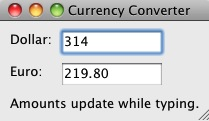
\includegraphics[width=0.2\textwidth]{html/hcar-reactive-banana-01.jpg}
\end{center}
%*endignore

Current development focuses on a more integrated notion of time and dynamic event switching.

\FurtherReading
\begin{compactitem}
\item Project homepage: \url{http://haskell.org/haskellwiki/Reactive-banana}
\item Example code: \url{http://haskell.org/haskellwiki/Reactive-banana/Examples}
\item Cabal package: \url{http://hackage.haskell.org/package/reactive-banana}
\item Developer blog:  \url{http://apfelmus.nfshost.com/blog.html}
\end{compactitem}
\end{hcarentry}
